\scanpage{88}
5.1.84

Soit $X$ une surface compacte, munie
d'un graphe topologique $X_1\subset X$ la
décomposant cellulairement. [On s'intéressera
plus particulièrement au cas où
\deleted{\unsure{tous}} les vts de $X_1$ sont d'ordre pair, p.e.
$(X,X_1)$ est un syst. de pseudo-droites
ds un plan \deleted{\unsure{p}} projectif réel topologique.]
\deleted{Soit} Un cercle topologique $D\subset X$ sera dit
``en \unsure{posit.}, \unsure{standard|standart}'' (p.r. à $X_1$), s'il
\deleted{\unsure{n'est en}} rencontre $X_1$, et si pour $\forall$
$a\in X_1\cap D$, \deleted{$D$ \uline{croise} \unsure{toutes les}} $a$ est un
pt d'ordre pair de $X_1$, et $D$ \uline{croise} ttes
branches de $X_1$ en $a$. On dit que deux
tels $D,D'$ sont ``en $=$ \unsure{position relative}''
ou sont \uline{isotopes}, si on peut passer
\inserted{(par des paramétrisations continues $D\simeq\unsure{\mathrm U|\mathrm U_1}$, $D'\simeq\unsure{\mathrm U|\mathrm U_1}$)}
de $D$ à $D'$ par une ``isotopie'', au cours
de laquelle, non seulement les positions
intermédiaires $D_t$ sont en position st.
mais en plus $D_t\cap S(\unsure{K|X})$ reste constant.
Il f. et s. pour cela que, \deleted{\unsure{pour}} \inserted{désignant} par
$\unsure{\Phi|\mathcal F}(D)$ l'ens. des facettes de $(X,X_1)$ rencontrées
par $D$, que l'on ait $\unsure{\Phi|\mathcal F}(D)=\unsure{\Phi|\mathcal F}(D')$. Il f. et s.
aussi qu'il existe une famille à un
paramètre $f_t$ $(0\leq t\leq1)$ d'autom. de
$(X,X_1)$, avec $f_0=\mathrm{id}$, et $f_1(D)=D'$.

On définit une notion de \uline{balayage} d'une
p.r. au dessus d'un sommet \uline{pair} de $X_1$,
comme dans le cas des syst. de ps. dr.,
et une notion correspondante de
spécialisation vers un sommet. \deleted{Également,
la notion de}
Pour $D$ donné, les op. de spéc. et de
généralis. à partir de $D$ se \unsure{repèrent}
encore p. des ``arcs de \deleted{balayage} \inserted{transition}'', sur
\deleted{\unsure{de}} la réu. $\widetilde D$ des rives de $D$, qui
\figure{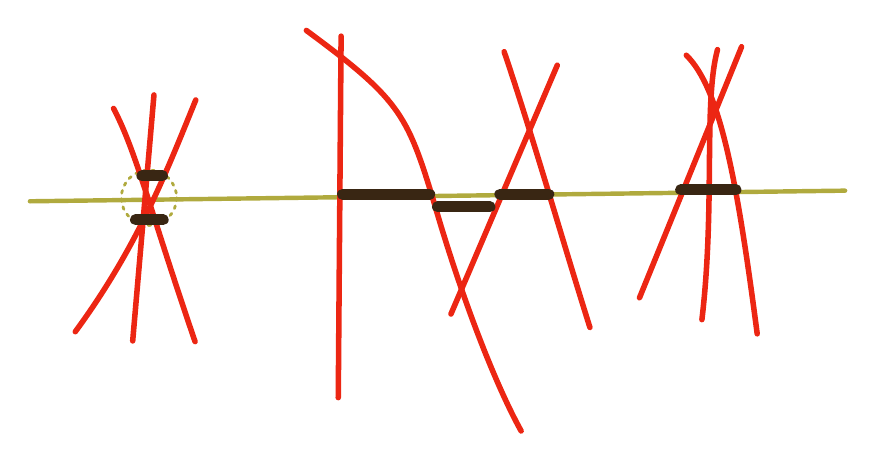
\begin{tikzpicture}[x=.009cm,y=-.009cm,line cap=round,line join=round]
\draw[yellow!65!black,line width=1.6pt](1600,1200)--(2750,1185);
\draw[yellow!65!black,line width=1pt,dotted](1768,1195) circle(39);
\draw[red!70!brown,line width=2pt](1718,1069)..controls(1750,1130)and(1769,1211)..(1833,1398);
\draw[red!70!brown,line width=2pt](1775,1050)--(1745,1397);
\draw[red!70!brown,line width=2pt](1834,1057)..controls(1792,1160)and(1752,1264)..(1664,1384);
\draw[brown!30!black,line width=4pt](1758,1164)--(1787,1164) (1749,1226)--(1788,1226);
\draw[red!70!brown,line width=2pt](2039,967)--(2035,1477);
\draw[red!70!brown,line width=2pt](1990,959)..controls(2120,1055)and(2132,1076)..(2169,1198)..controls(2210,1340)and(2258,1461)..(2293,1524);
\draw[red!70!brown,line width=2pt](2344,1008)--(2194,1359);
\draw[red!70!brown,line width=2pt](2269,989)..controls(2310,1110)and(2350,1251)..(2390,1378);
\draw[brown!30!black,line width=4pt](2041,1190)--(2164,1190) (2175,1208)--(2249,1208) (2263,1190)--(2332,1190);
\draw[red!70!brown,line width=2pt](2526,994)..controls(2573,1040)and(2597,1165)..(2626,1387);
\draw[red!70!brown,line width=2pt](2570,986)..controls(2550,1060)and(2567,1206)..(2548,1367);
\draw[red!70!brown,line width=2pt](2604,982)--(2460,1336);
\draw[brown!30!black,line width=4pt](2518,1184)--(2596,1184);
\end{tikzpicture}}
forment, en se recollant, une
famille d'arcs \deleted{\unsure{puis}} \inserted{\unsure{dont les adh.}} sont deux à deux disjoints.
Il y a une notion de transport parallèle
pour $\widetilde D$, munie de sa structure de
contour \inserted{top.} naturelle (ou plutôt, pour
sa structure combinatoire) pour tte
généralis. de spéc. en gén., et aussi
\margin{87}
